\documentclass[12pt,compress]{beamer}
\usepackage{ifthen,verbatim}

\title{Progress in Pixelless Electron-Finding}
\author{Jim Pivarski}
\institute{Cornell University}
\date{21 July, 2006}

\setbeamertemplate{navigation symbols}{}
\setbeamertemplate{headline}{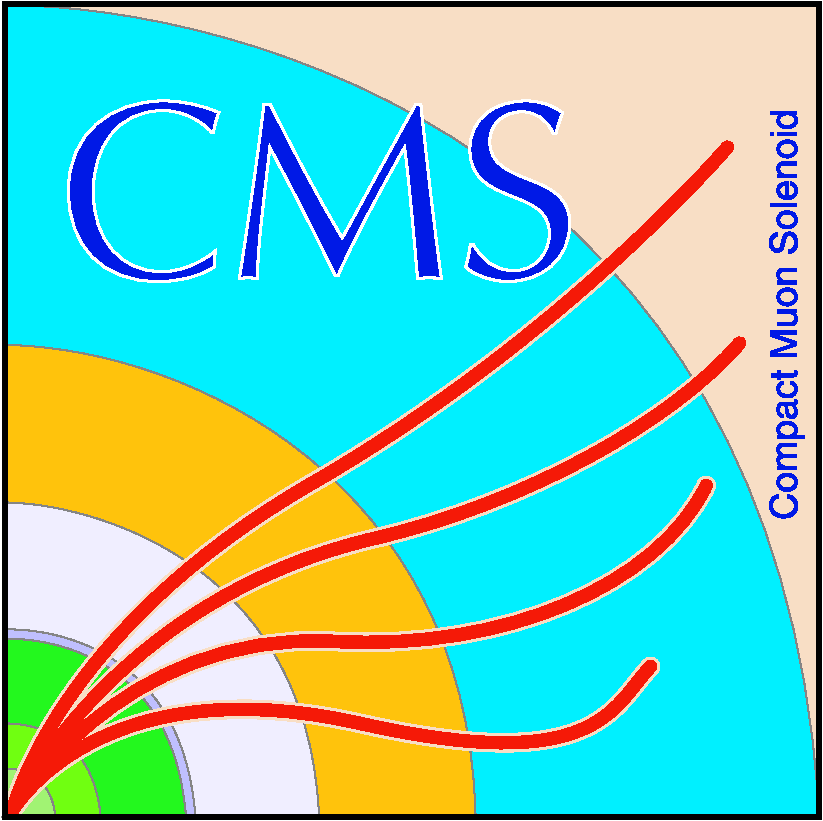
\includegraphics[height=1 cm]{cmslogo} \hfill
\begin{minipage}{8 cm}
\vspace{-0.75 cm} \small
\begin{center}
\ifthenelse{\equal{\insertpagenumber}{0}}{}{\insertsection\ (\insertpagenumber/\pageref{numpages})}
\end{center}
\end{minipage} \hfill 
\includegraphics[height=1 cm]{lepplogo}}

\xdefinecolor{verylightgray}{rgb}{0.95,0.95,0.95}
\beamertemplateshadingbackground{verylightgray}{white}

\begin{document}
\addtocounter{page}{-1}
\frame{\titlepage}
\section*{Pixelless Electrons --- Jim Pivarski}

\begin{frame}
\begin{description}\setlength{\itemsep}{0.3 cm}
\item[last time:]<1-> submitted dummy producer and object (SiStripElectronProducer and SiStripElectron)
\item<1-> implemented simple ``band'' algorithm
\item[today:]<2-> added useful features to algorithm
\item<2-> output TrackCandidates and fit tracks (KFFinalFit with material)
\item<2-> produced diagnostic plots
\item[however:]<3-> tracking efficiency is 3\%
\item<3-> electrons and fitted tracks are not yet associated
\end{description}

\end{frame}

\begin{frame}
\frametitle{Band Algorithm}

\vspace{-0.5 cm}
\begin{center}
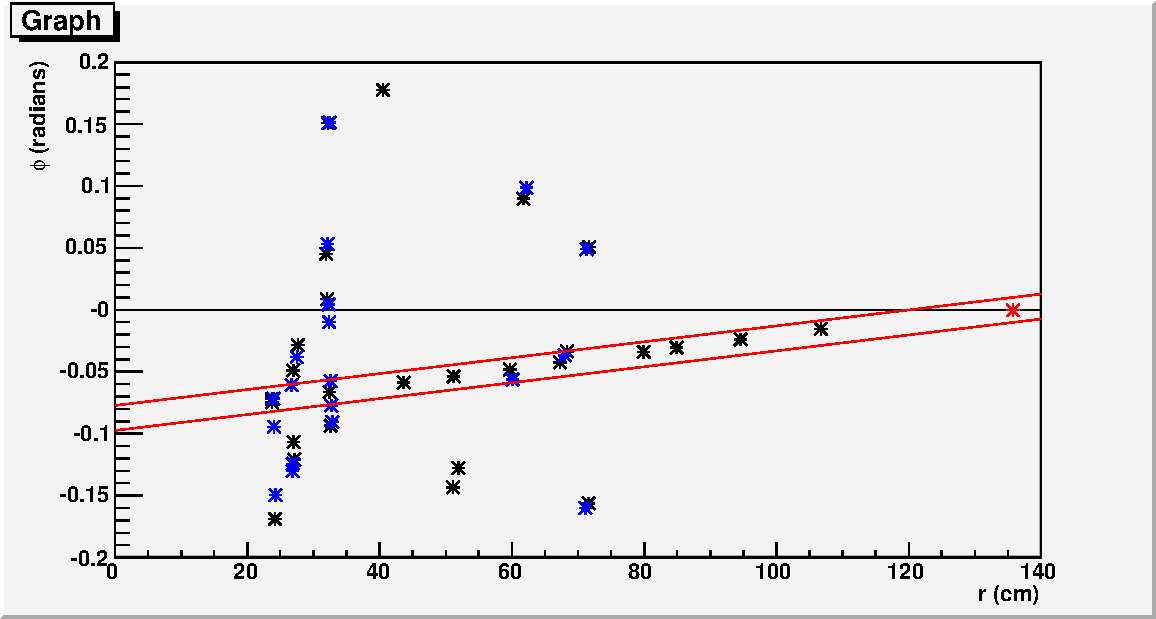
\includegraphics[width=0.8\linewidth]{event_display_banded}
\end{center}

\vspace{-0.5 cm}
\begin{itemize}
\item plot hit $\phi$ versus hit radius (mentally)
\item project a line from SuperCluster position and energy
\item count hits within a $\Delta \phi$ band
\end{itemize}
\end{frame}

\begin{frame}
\frametitle{New Features in SiStripElectronProducer}
\begin{itemize}\setlength{\itemsep}{0.5 cm}
\item linear fit $z(r)$ of stereo hits determine vertex $z$ and $\eta$
\item $\Delta z$ window provides more hit discrimination
\item linear fit to $\phi(r)$ yields $\phi_0$, average $p_T$, and $\chi^2$
\item we try both charge hypotheses but accept only one
\item hits associated with each SuperCluster are disjoint sets
\item output hits and trajectory as a TrackCandidate for fitting
\end{itemize}
\end{frame}

\begin{frame}[fragile]
\frametitle{Sample .cfg excerpt}

\hspace{-0.4 cm}\begin{minipage}{\linewidth}
\scriptsize
\begin{verbatim}
# Find the electrons
include "RecoEgamma/EgammaElectronProducers/data/findElectronsInSiStrips.cfi"

# TrackProducer
include "RecoTracker/TrackProducer/data/CTFFinalFitWithMaterial.cfi"
replace CTFWMaterial.src = "findElectronsInSiStrips"

# Associate fitted tracks with SiStripElectrons to make reco::Electrons (future)
include "RecoEgamma/EgammaElectronProducers/data/buildElectronObjects.cfi"

path p = {
    findElectronsInSiStrips,
    CTFWMaterial,
    buildElectronObjects    # (future)
  }
\end{verbatim}
\end{minipage}
\begin{center}
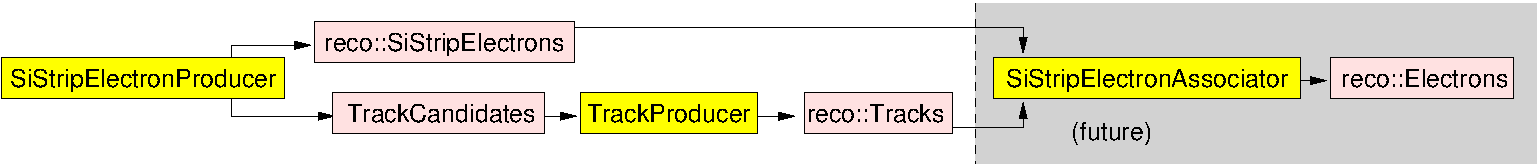
\includegraphics[width=\linewidth]{objects}
\end{center}
\end{frame}

\begin{frame}
\frametitle{Diagnostic Plots}

\vspace{-0.5 cm}
\begin{center}
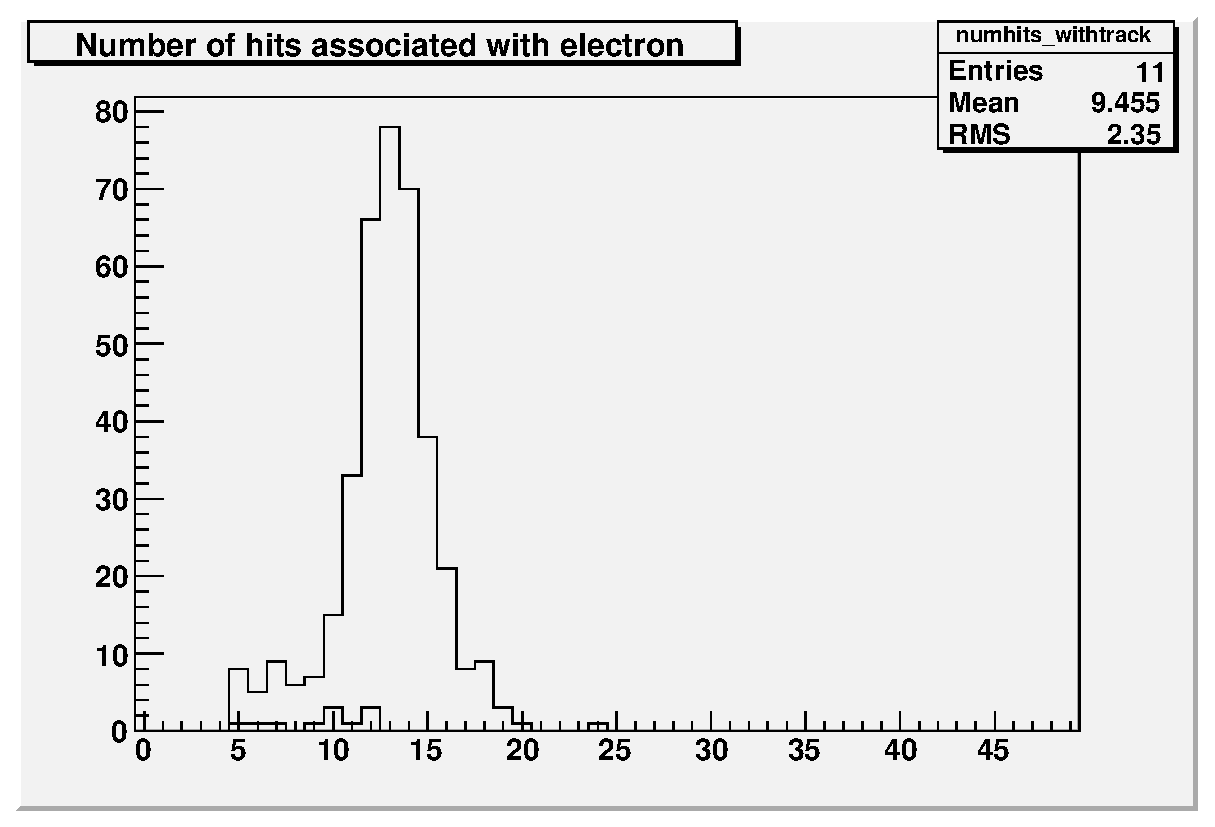
\includegraphics[width=0.6\linewidth]{numhits_withtrack_overlay}
\end{center}

\vspace{-0.3 cm}
\begin{itemize}
\item Using Chris Jones's new FWCore/TFWLiteSelector
\item 50 GeV, $\eta=0$ electron gun, $\Delta \phi$ band width = 0.01~rad
\item 400 events, 378 identified electrons, 11 fitted tracks
\end{itemize}
\end{frame}

\begin{frame}
\frametitle{Late-breaking news:}

I brought this up at the tracking meeting, and they pointed out two things:

\vspace{0.25 cm}
\begin{itemize}\setlength{\itemsep}{0.25 cm}
\item We need to sort hits given to the tracker.
\item We need to reduce the number of noise hits.
\end{itemize}

\vspace{0.25 cm}
This will probably make a difference.

\end{frame}

\begin{frame}
\frametitle{\only<1>{Before}\only<2>{After} track fitting \only<1>{(reco::SiStripElectrons)}\only<2>{(reco::Tracks)}}
\alt<1>{Linear fit of hits to $\phi(r)$ yields $\phi_0$ and average $p_T$}{Full track-fit, evaluated at the closest point to the origin}
\begin{center}
\begin{tabular}{p{0.45\linewidth} p{0.45\linewidth}}
\begin{minipage}{\linewidth}
\alt<1>{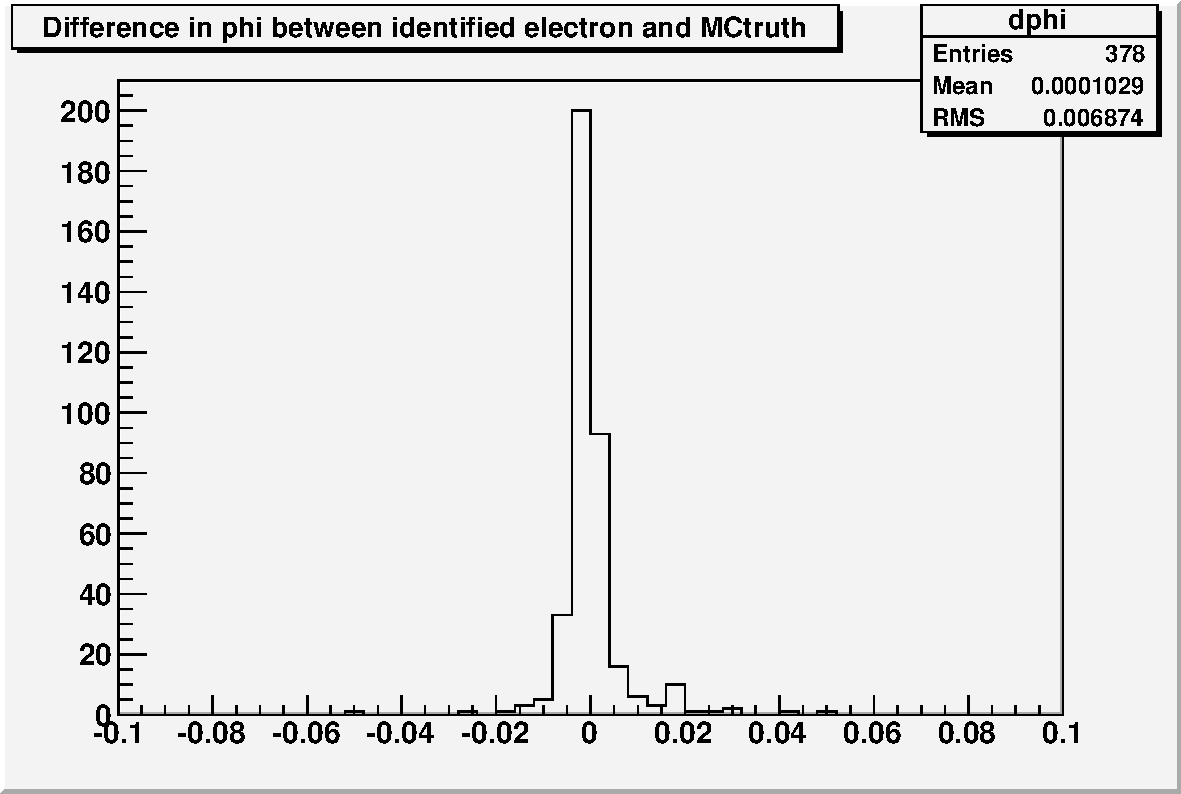
\includegraphics[width=\linewidth]{dphi}}{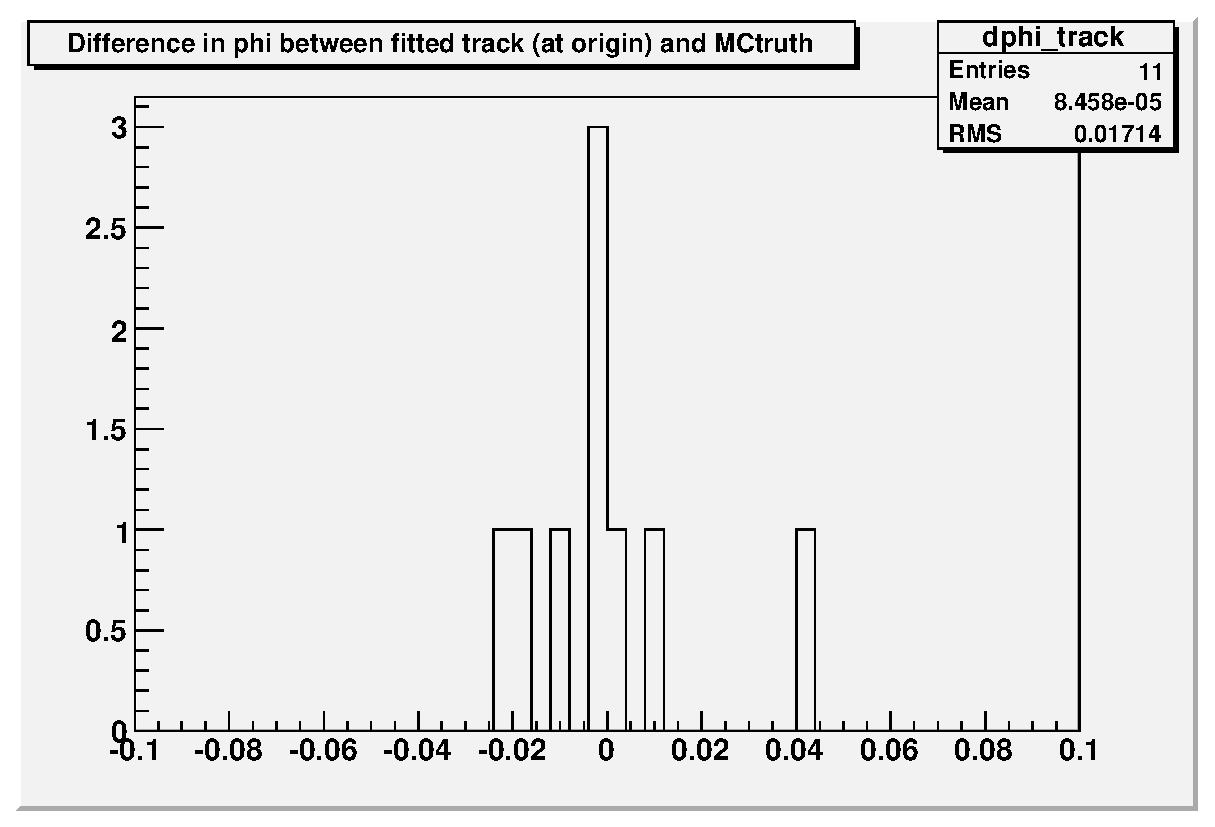
\includegraphics[width=\linewidth]{dphi_track}}
\end{minipage} &
\begin{minipage}{\linewidth}
\alt<1>{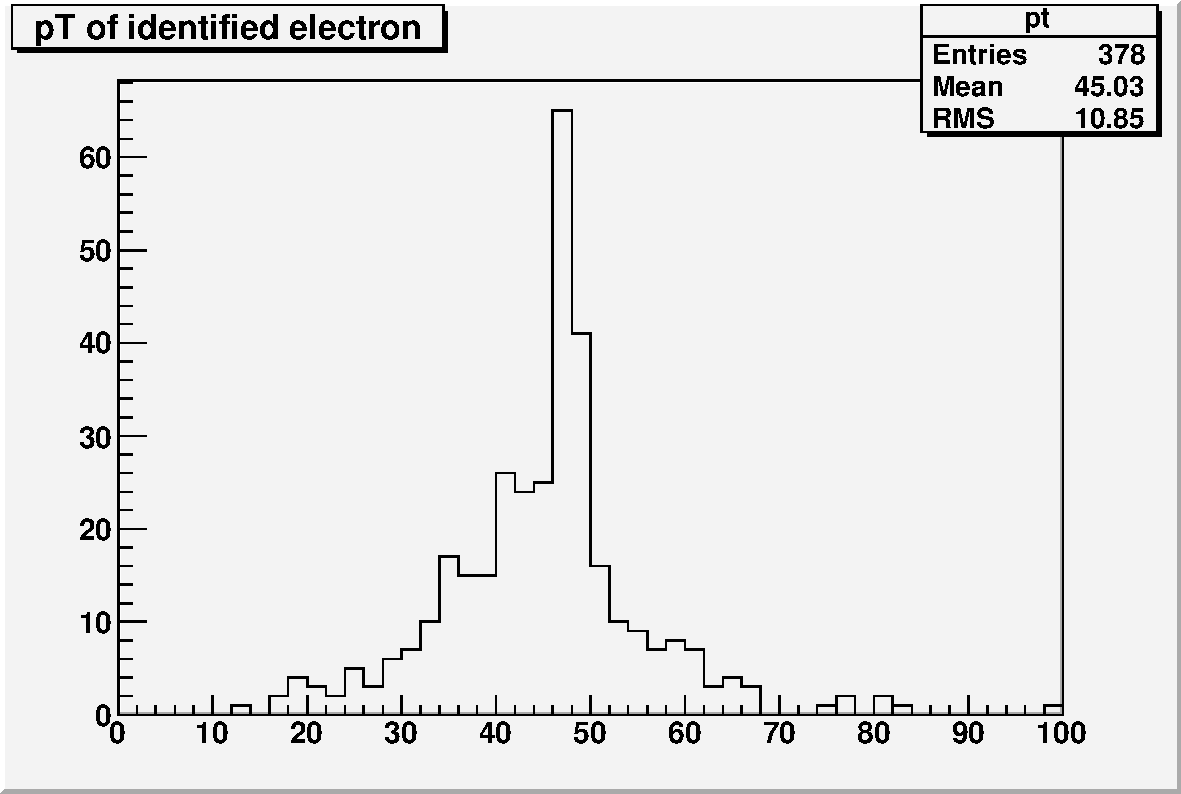
\includegraphics[width=\linewidth]{pt}}{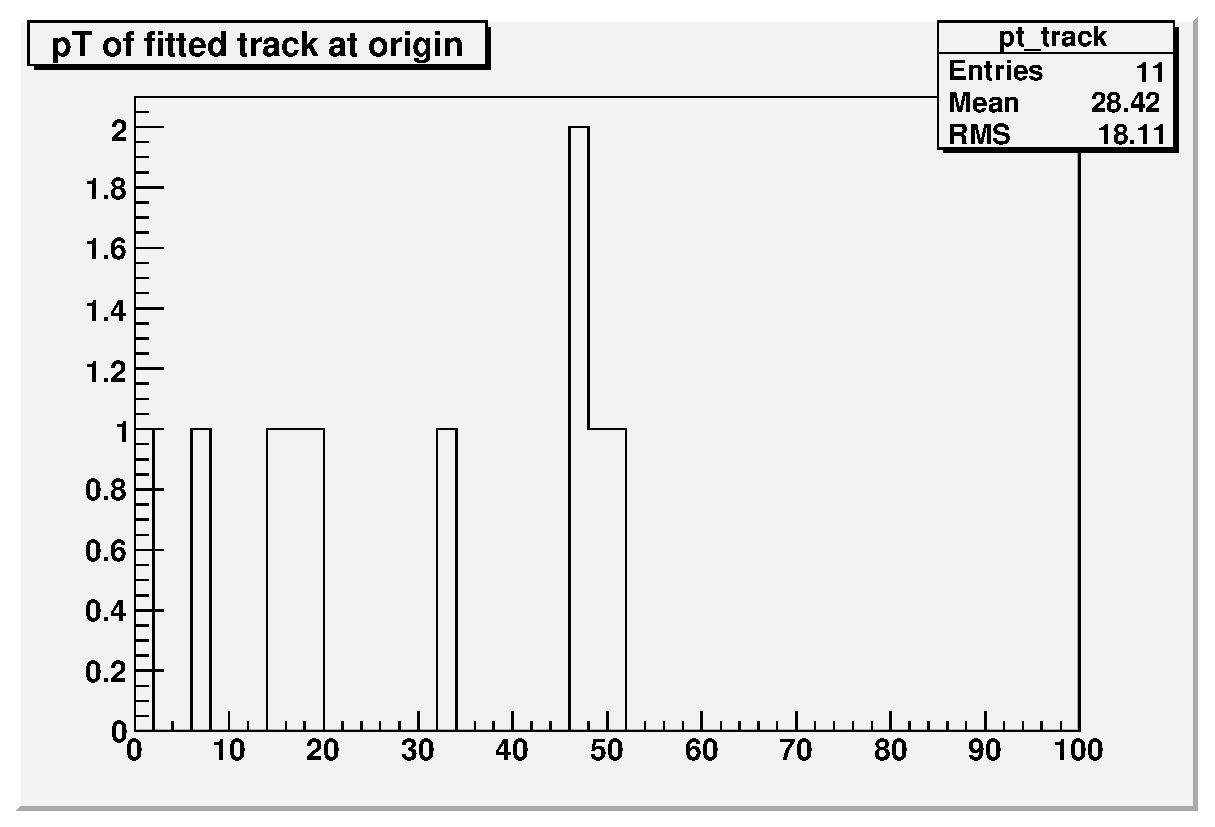
\includegraphics[width=\linewidth]{pt_track}}
\end{minipage} \\
& \\
\begin{minipage}{\linewidth}
\begin{center}
fitted $\phi_0$ $-$ true $\phi_0$
\end{center}
\end{minipage} &
\begin{minipage}{\linewidth}
\begin{center}
fitted $p_T$ for 50 GeV
\end{center}
\end{minipage}
\end{tabular}
\end{center}
\end{frame}

\begin{frame}
\frametitle{\only<1>{Before}\only<2>{After} track fitting \only<1>{(reco::SiStripElectrons)}\only<2>{(reco::Tracks)}}
\alt<1>{Linear fit of stereo hits to $z(r)$ yields $z_0$ and $\eta$}{Full track-fit, evaluated at the closest point to the origin}
\begin{center}
\begin{tabular}{p{0.45\linewidth} p{0.45\linewidth}}
\begin{minipage}{\linewidth}
\alt<1>{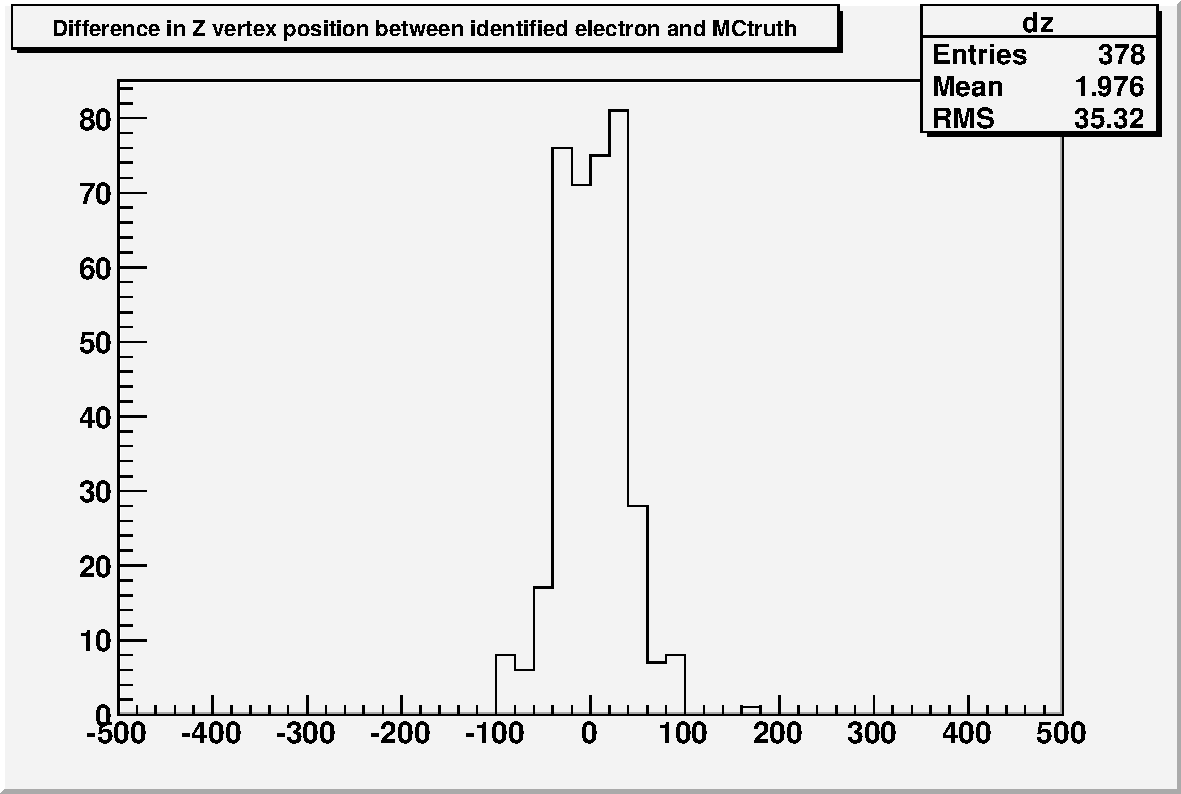
\includegraphics[width=\linewidth]{dz}}{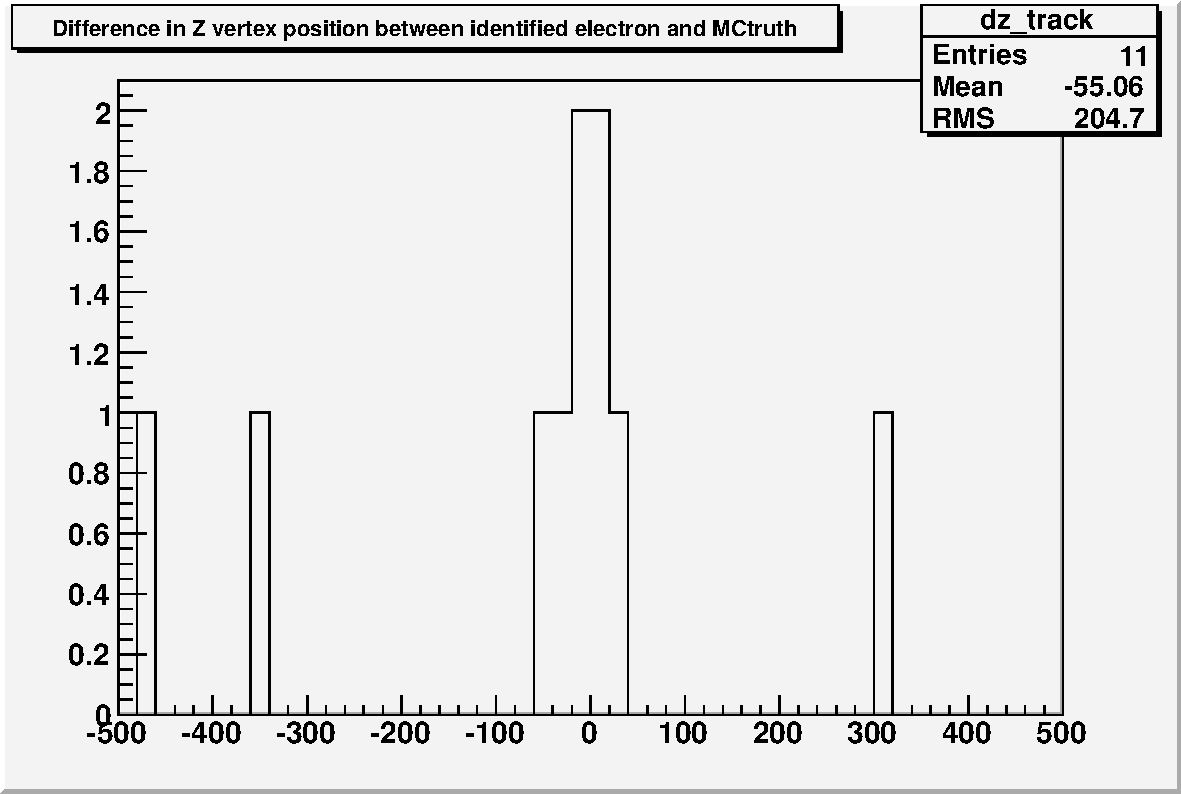
\includegraphics[width=\linewidth]{dz_track}}
\end{minipage} &
\begin{minipage}{\linewidth}
\alt<1>{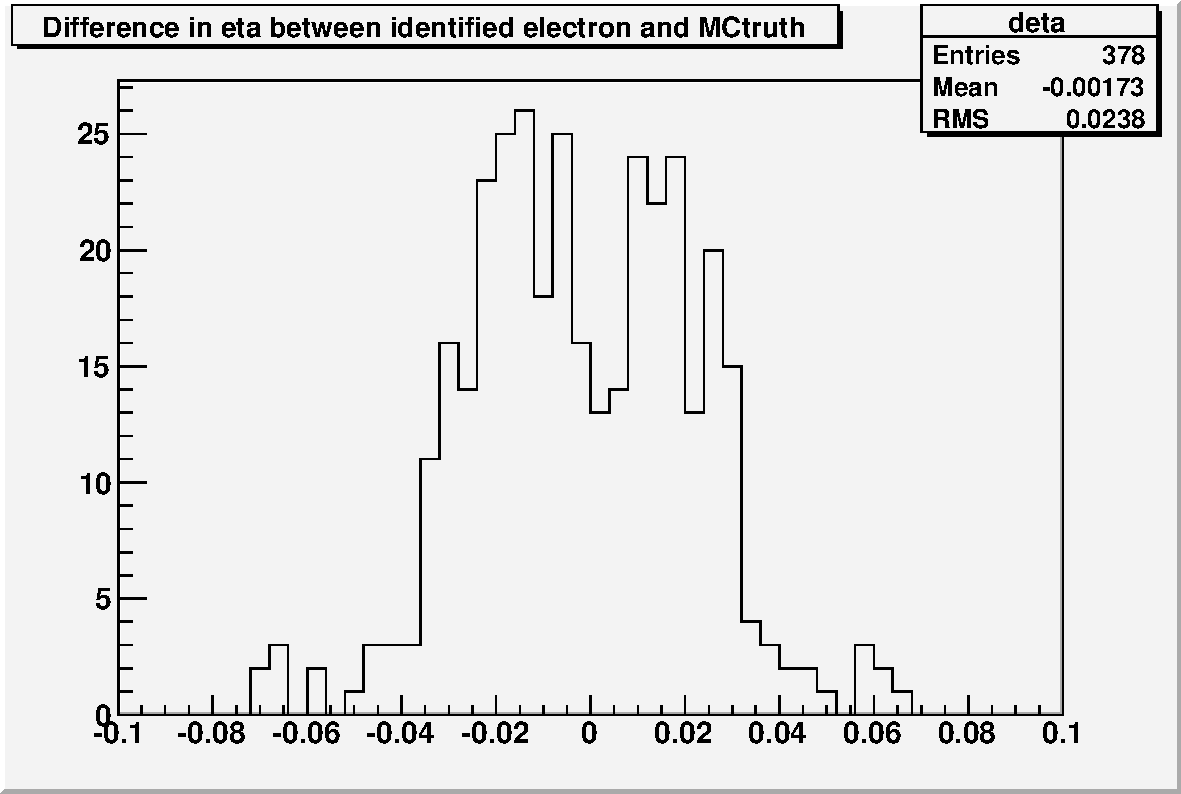
\includegraphics[width=\linewidth]{deta}}{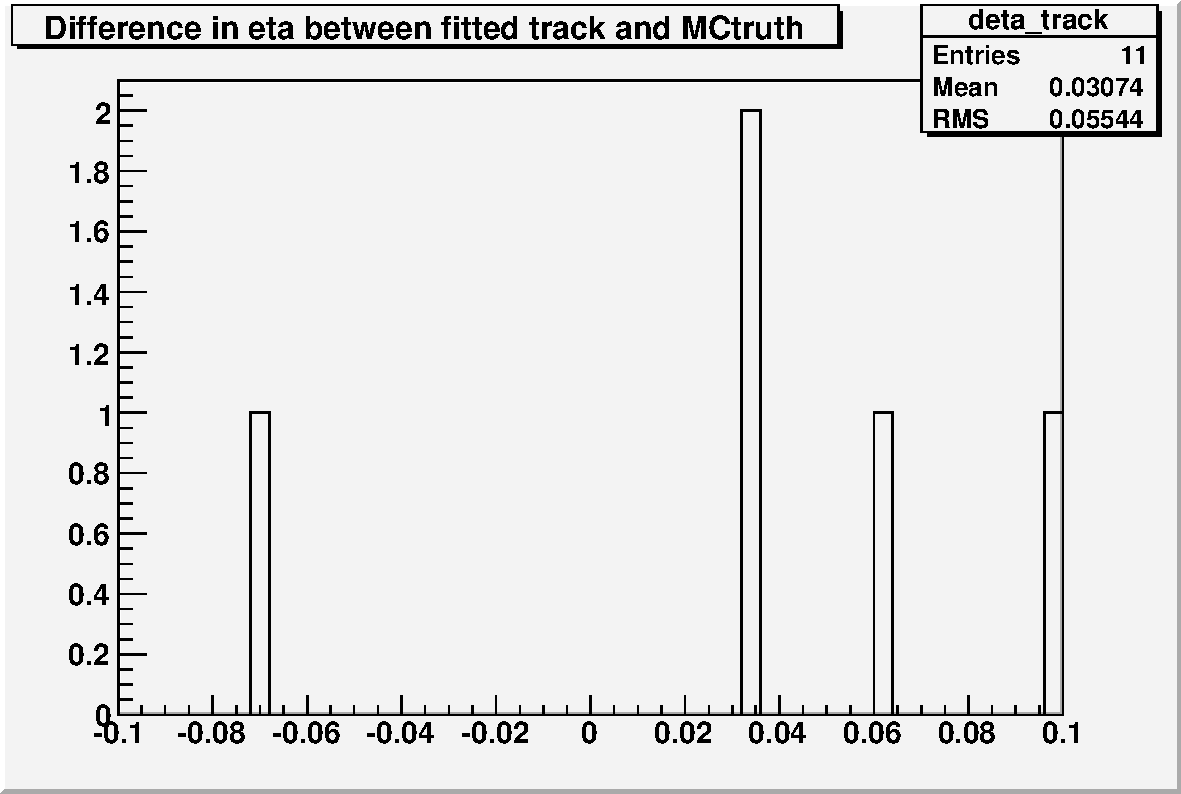
\includegraphics[width=\linewidth]{deta_track}}
\end{minipage} \\
& \\
\begin{minipage}{\linewidth}
\begin{center}
fitted $z_0$ $-$ true $z_0$ (mm?)
\end{center}
\end{minipage} &
\begin{minipage}{\linewidth}
\begin{center}
fitted $\eta$ for $\eta=0$
\end{center}
\end{minipage}
\end{tabular}
\end{center}
\end{frame}

\begin{frame}[fragile]
\frametitle{What units is the vertex in, anyway?}
\begin{minipage}{\linewidth}
\scriptsize
\begin{verbatim}
module VtxSmeared = VertexGenerator {
    string type = "IOMC/EventVertexGenerators/GaussianEventVertexGenerator"
    double SigmaX = 0.015
    double SigmaY = 0.015
    double SigmaZ = 53.0  // in mm (as in COBRA/OSCAR)
}
\end{verbatim}
\end{minipage}

\vspace{0.5 cm} \hspace{-0.8 cm}
Output of HepMC::GenParticle::CreationVertex().z():

\vspace{-0.3 cm}
\begin{center}
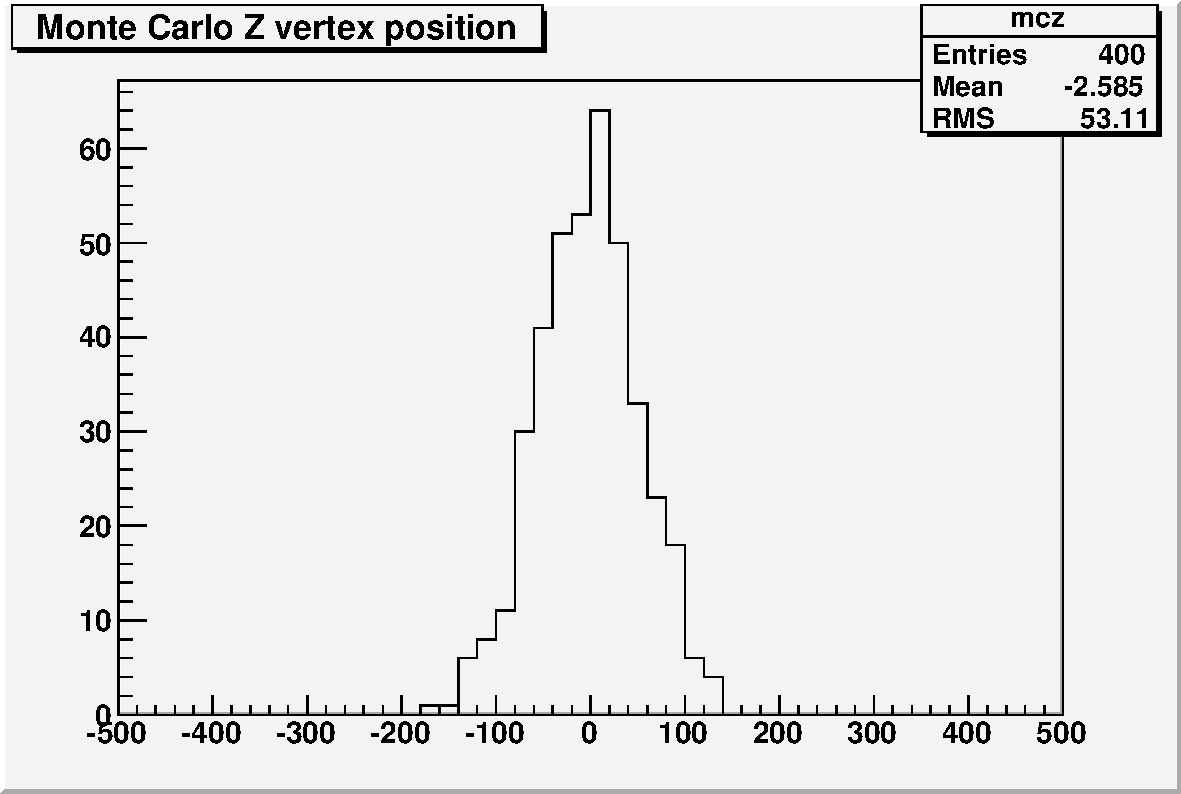
\includegraphics[width=0.5\linewidth]{mcz}
\end{center}
\end{frame}

\begin{frame}
\frametitle{$\chi^2$ values are very poor}
\begin{center}
\begin{tabular}{p{0.45\linewidth} p{0.45\linewidth}}
\begin{minipage}{\linewidth}
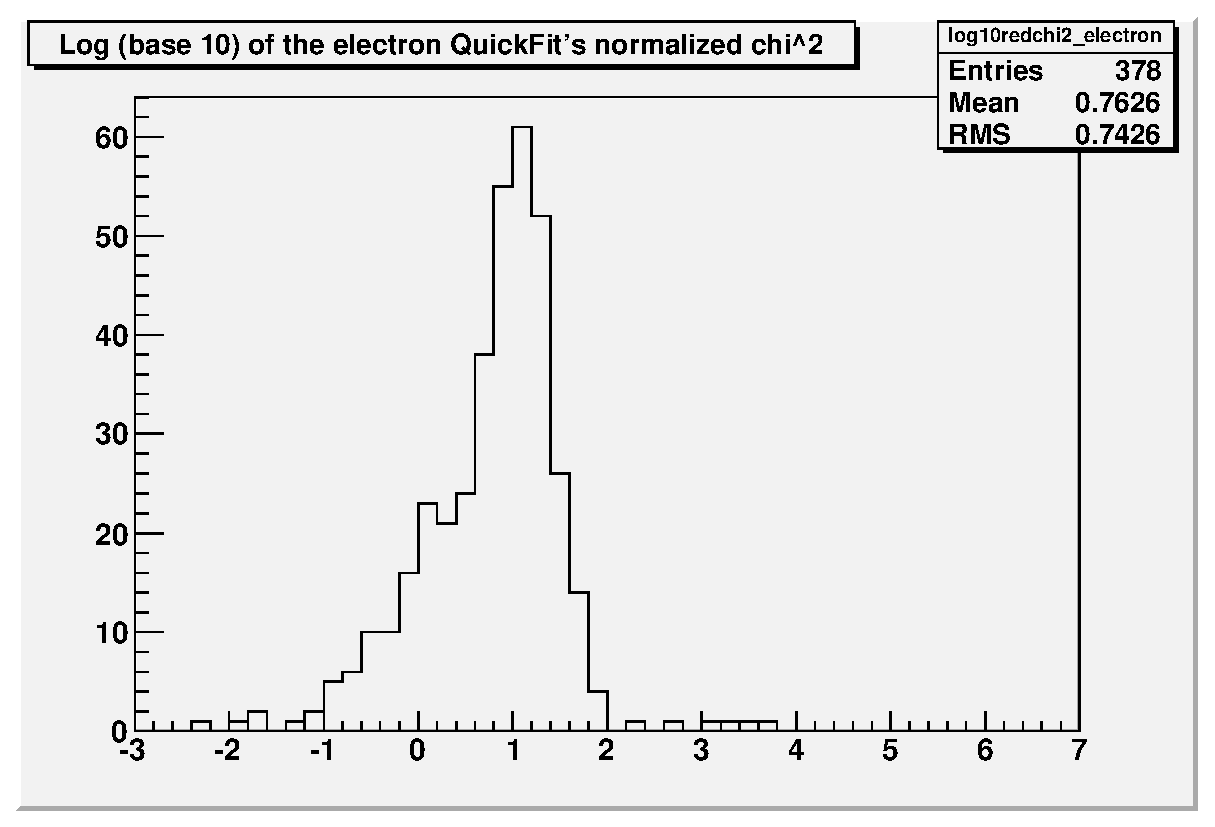
\includegraphics[width=\linewidth]{log10redchi2_electron}
\end{minipage} &
\begin{minipage}{\linewidth}
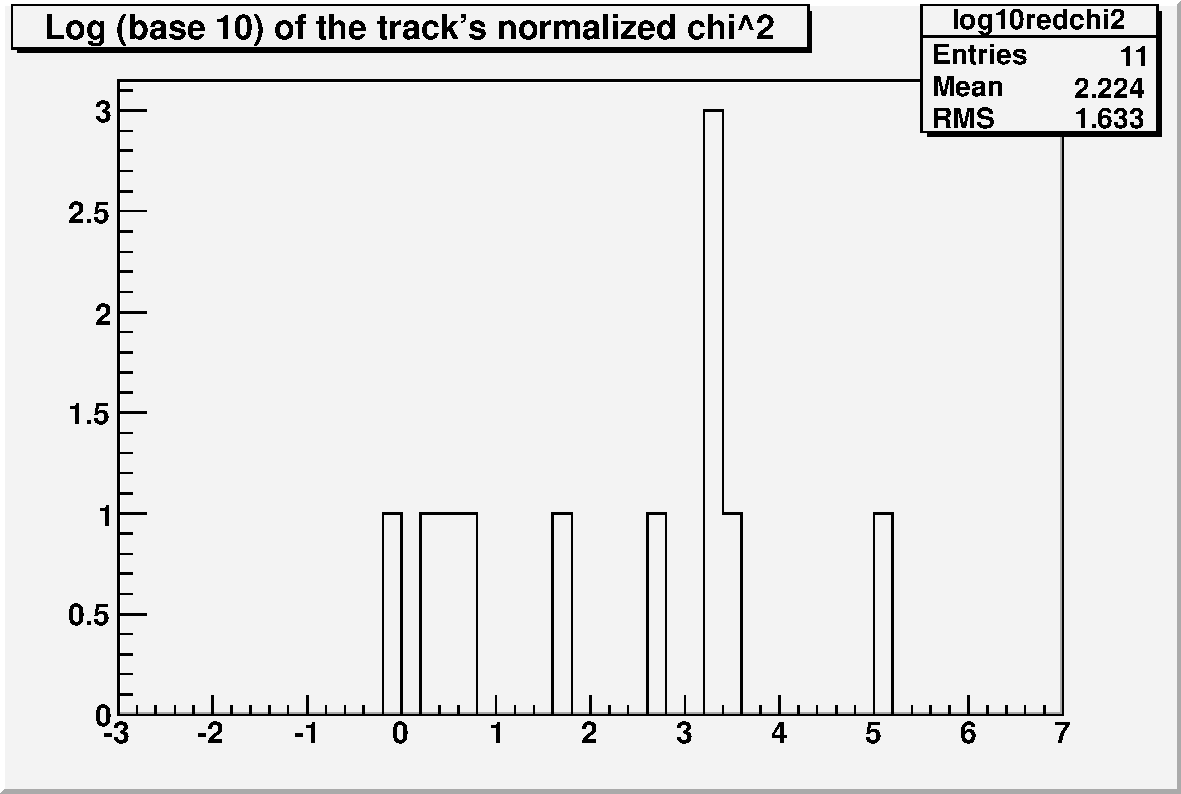
\includegraphics[width=\linewidth]{log10redchi2}
\end{minipage} \\
& \\
\begin{minipage}{\linewidth}
\begin{center}
$\log_{10}(\chi^2/N_{\mbox{\scriptsize dof}})$ of linear fit
\end{center}
\end{minipage} &
\begin{minipage}{\linewidth}
\begin{center}
$\log_{10}(\chi^2/N_{\mbox{\scriptsize dof}})$ of full fit
\end{center}
\end{minipage} \\
& \\
\begin{minipage}{\linewidth}
\begin{center}
(reco::SiStripElectrons)
\end{center}
\end{minipage} &
\begin{minipage}{\linewidth}
\begin{center}
(reco::Tracks)
\end{center}
\end{minipage}
\end{tabular}
\end{center}
\end{frame}

%% \begin{frame}[fragile]
%% \frametitle{What's happening to those tracks?}
%% \begin{minipage}{\linewidth}
%% \tiny
%% \begin{verbatim}
%% %MSG-e TrackingTools/TrackFitters:  TrackProducer:CTFWMaterial 
%%        20-Jul-2006 14:48:42 EDT 1/397
%%  SOMETHING WRONG !
%% KFTrajectoryFitter: predicted tsos not valid!
%% current TSOS: global parameters
%% x =        60.056      1.75458      7.61882
%% p =       15.6024    0.0627532    0.0192975
%% global error
%%    0.00441064   0.00367666  -0.00123642   -0.0119792     0.119831
%%    0.00367666   0.00726461  -0.00144864   -0.0236283     0.236437
%%   -0.00123642  -0.00144864   0.00038832   0.00471968    -0.047212
%%    -0.0119792   -0.0236283   0.00471968    0.0769768    -0.770017
%%      0.119831     0.236437    -0.047212    -0.770017      7.70519
%% local parameters (q/p,v',w',v,w)
%%     0.0640923   -0.0891444    0.0101923     -4.00179     -1.21915
%% local error
%%    0.00441064 -0.000872564   0.00379766 -3.92563e-06     0.120435
%%  -0.000872564  0.000172742  -0.00075066  1.55518e-06   -0.0238357
%%    0.00379766  -0.00075066   0.00754605 -1.29175e-07     0.242177
%%  -3.92563e-06  1.55518e-06 -1.29175e-07  2.52719e-05 -1.68039e-06
%%      0.120435   -0.0238357     0.242177 -1.68039e-06      7.78295

%% %MSG-e TrackingTools/TrackFitters:  TrackProducer:CTFWMaterial 
%%        20-Jul-2006 14:48:42 EDT 1/397
%% next Surface:  (27.0362,3.06581,7.5766) 
%% \end{verbatim}
%% \end{minipage}
%% \end{frame}

%% \begin{frame}
%% \frametitle{What's happening to those tracks?}
%% \begin{center}
%% 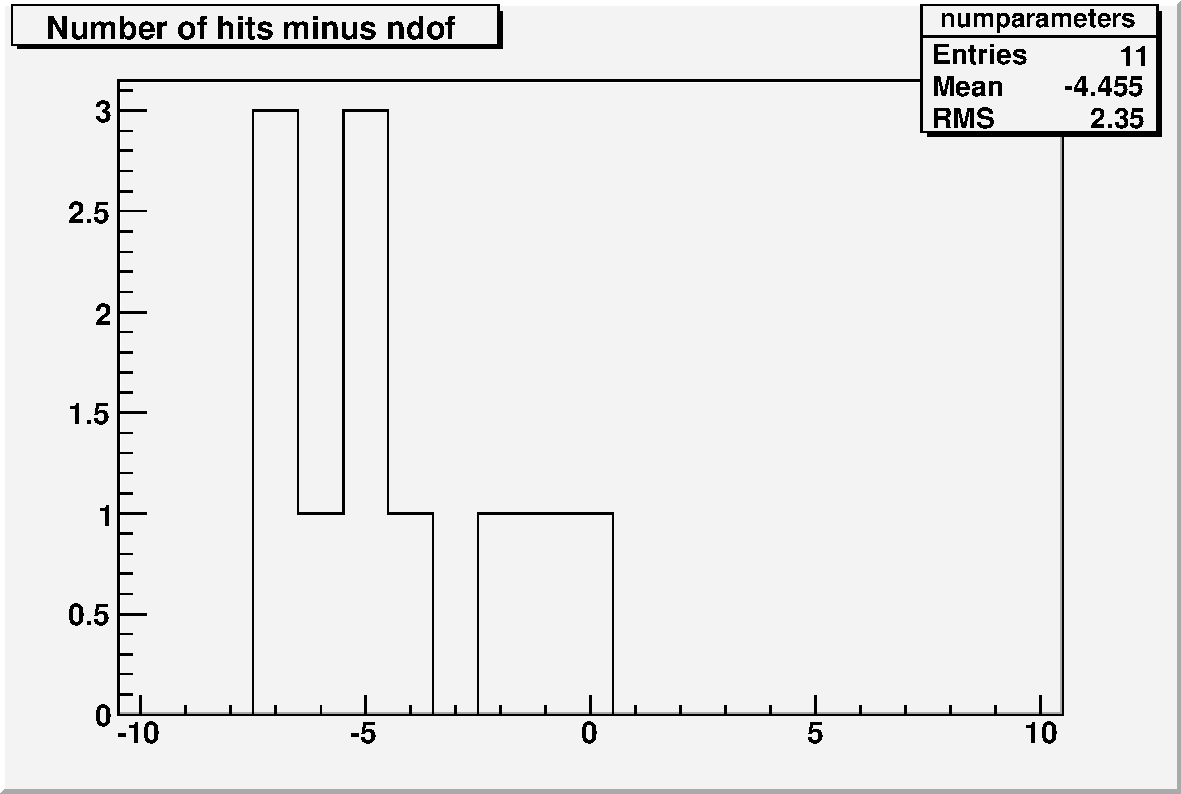
\includegraphics[width=0.9\linewidth]{numparameters}
%% \end{center}
%% \end{frame}

\begin{frame}
\frametitle{Next steps}

Track seeding
\begin{itemize}\setlength{\itemsep}{0.25 cm}
\item Ask tracking experts about track-fitting failures
\item Ask Ursula and Claude how they are seeding tracks
\item Write track-electron associator
\end{itemize}

\vfill
Hit matching
\begin{itemize}\setlength{\itemsep}{0.25 cm}
\item Apply it to multi-electron (physics!) events, QCD
\item Study hit distributions and track efficiency in a realistic environment
\item Improve electron identification algorithm
\end{itemize}
\label{numpages}
\end{frame}

%% \section*{Additional material}

%% \begin{frame}[fragile]
%% \frametitle{How we make SiStrip hits and set up tracking}
%% \tiny
%% \begin{verbatim}
%% # tracker geometry
%% include "Geometry/TrackerGeometryBuilder/data/trackerGeometry.cfi"

%% # tracker numbering
%% include "Geometry/TrackerNumberingBuilder/data/trackerNumberingGeometry.cfi"

%% # standard geometry
%% include "Geometry/CMSCommonData/data/cmsIdealGeometryXML.cfi"

%% # magnetic field
%% include "MagneticField/Engine/data/volumeBasedMagneticField.cfi"

%% # make SiStrip rechits
%% include "RecoLocalTracker/SiStripRecHitConverter/data/StripCPEfromTrackAngle.cfi"
%% include "RecoLocalTracker/SiStripClusterizer/data/SiStripClusterizer.cfi"
%% include "RecoLocalTracker/SiStripRecHitConverter/data/SiStripRecHitConverter.cfi"
%% \end{verbatim}

%% \normalsize
%% Add ThreeThresholdClusterizer and LocalMeasurementConverter to path

%% \end{frame}

%% \begin{frame}[fragile]
%% \tiny
%% \begin{verbatim}
%% # KFUpdatoerESProducer
%% include "TrackingTools/KalmanUpdators/data/KFUpdatorESProducer.cfi"

%% # Chi2MeasurementEstimatorESProducer
%% include "TrackingTools/KalmanUpdators/data/Chi2MeasurementEstimatorESProducer.cfi"

%% # KFTrajectoryFitterESProducer
%% include "TrackingTools/TrackFitters/data/KFTrajectoryFitterESProducer.cfi"

%% # KFTrajectorySmootherESProducer
%% include "TrackingTools/TrackFitters/data/KFTrajectorySmootherESProducer.cfi"

%% # KFFittingSmootherESProducer
%% include "TrackingTools/TrackFitters/data/KFFittingSmootherESProducer.cfi"

%% # PropagatorWithMaterialESProducer
%% include "TrackingTools/MaterialEffects/data/MaterialPropagator.cfi"

%% # PropagatorWithMaterialESProducer
%% include "TrackingTools/MaterialEffects/data/OppositeMaterialPropagator.cfi"

%% # stripCPE
%% include "RecoLocalTracker/SiStripRecHitConverter/data/StripCPEfromTrackAngle.cfi"

%% # pixelCPE
%% include "RecoLocalTracker/SiPixelRecHits/data/PixelCPEParmError.cfi"

%% #TransientTrackingBuilder
%% include "RecoTracker/TransientTrackingRecHit/data/TransientTrackingRecHitBuilder.cfi"

%% # TrackProducer
%% include "RecoTracker/TrackProducer/data/CTFFinalFitWithMaterial.cfi"
%% replace CTFWMaterial.src = "findElectronsInSiStrips"
%% \end{verbatim}
%% \end{frame}

%% \begin{frame}[fragile]
%% \frametitle{C++ code}
%% \tiny
%% \begin{verbatim}
%% // GlobalTrajectoryParameters evaluated at the position of the innerhit
%% GlobalPoint position = tracker_p_->idToDet(
%%    innerhit->geographicalId())->surface().toGlobal(innerhit->localPosition());

%% // Now we can construct a trajectory momentum out of linear fits to hits
%% GlobalVector momentum = GlobalVector(pT*cos(phi), pT*sin(phi), pZ);

%% // Initial uncertainty for tracking
%% AlgebraicSymMatrix errors(5,1);  // makes identity 5x5 matrix, indexed from (1,1) to (5,5)
%% errors(1,1) = 3.;      // uncertainty**2 in 1/momentum
%% errors(2,2) = 0.01;    // uncertainty**2 in lambda (lambda == pi/2 - polar angle theta)
%% errors(3,3) = 0.0001;  // uncertainty**2 in phi
%% errors(4,4) = 0.01;    // uncertainty**2 in x_transverse (where x is in cm)
%% errors(5,5) = 0.01;    // uncertainty**2 in y_transverse (where y is in cm)

%% TrajectoryStateOnSurface state(
%%    GlobalTrajectoryParameters(position, momentum, -1, magneticField_p_),
%%    CurvilinearTrajectoryError(errors),
%%    tracker_p_->idToDet(innerhit->geographicalId())->surface());

%% TrajectoryStateTransform transformer;
%% PTrajectoryStateOnDet* PTraj = transformer.persistentState(state, innerhit->geographicalId().rawId());
%% TrajectorySeed trajectorySeed(*PTraj, outputHits, alongMomentum);
%% trackCandidateOut.push_back(TrackCandidate(outputHits, trajectorySeed, *PTraj));
%% \end{verbatim}
%% \end{frame}

%% \begin{frame}[fragile]
%% \frametitle{Error messages: x and p look wrong\ldots}
%% \tiny
%% \begin{verbatim}
%% current TSOS: global parameters
%% x =      -68.0476      21.0676    -0.745468
%% p =      -2.89165     0.421055      1.02657
%% current TSOS: global parameters
%% x =       -42.292      57.3303     -12.3466
%% p =       -6.0335      9.23854     -2.01767
%% current TSOS: global parameters
%% x =       65.2933      28.2551     -3.31759
%% p =       7.38007      3.75951    0.0653902
%% current TSOS: global parameters
%% x =      -20.1964      25.6679      7.38585
%% p =      -0.11732    0.0388591  -0.00374432
%% current TSOS: global parameters
%% x =       60.9142     -27.7915      5.40479
%% p =       44.0689      -19.867     -2.28133
%% current TSOS: global parameters
%% x =       59.6496      6.08842      7.67884
%% p =       8.36302     0.454979    0.0255218
%% current TSOS: global parameters
%% x =       23.8705      6.12086     -3.97122
%% p =       1.47172     0.406813   -0.0235268
%% current TSOS: global parameters
%% x =       65.3329     -28.3907     -8.56305
%% p =       11.9033     -4.79491   -0.0706362
%% current TSOS: global parameters
%% x =      -29.9235     -11.0507     -3.43524
%% p =     -0.153422    0.0254676   0.00385046
%% \end{verbatim}
%% \end{frame}

\end{document}
